\subsection{Datenanalyse}
\label{subsec:revpar_analyse}

Wie bereits in Abschnitt \emph{\nameref{subsec:Datenanalyse}} erläutert wurde, ist die Datenanalyse eine der essenziellsten Komponenten bei der Modellierung eines Modells. Im Folgenden wird daher untersucht, welche hotelspezifischen Daten vorhanden sind und wie sie effektiv genutzt werden können.
\newline
\newline
Als erster Schritt soll erforscht werden, ob der gesamte Zeitraum des Datensatzes valide ist und verwendet werden kann. Dazu wird zunächst der durchschnittliche normierte RevPAR, repräsentiert durch die Spalte \emph{target}, mit den einzelnen Jahren verglichen.

\begin{figure}[h]
    \centering
    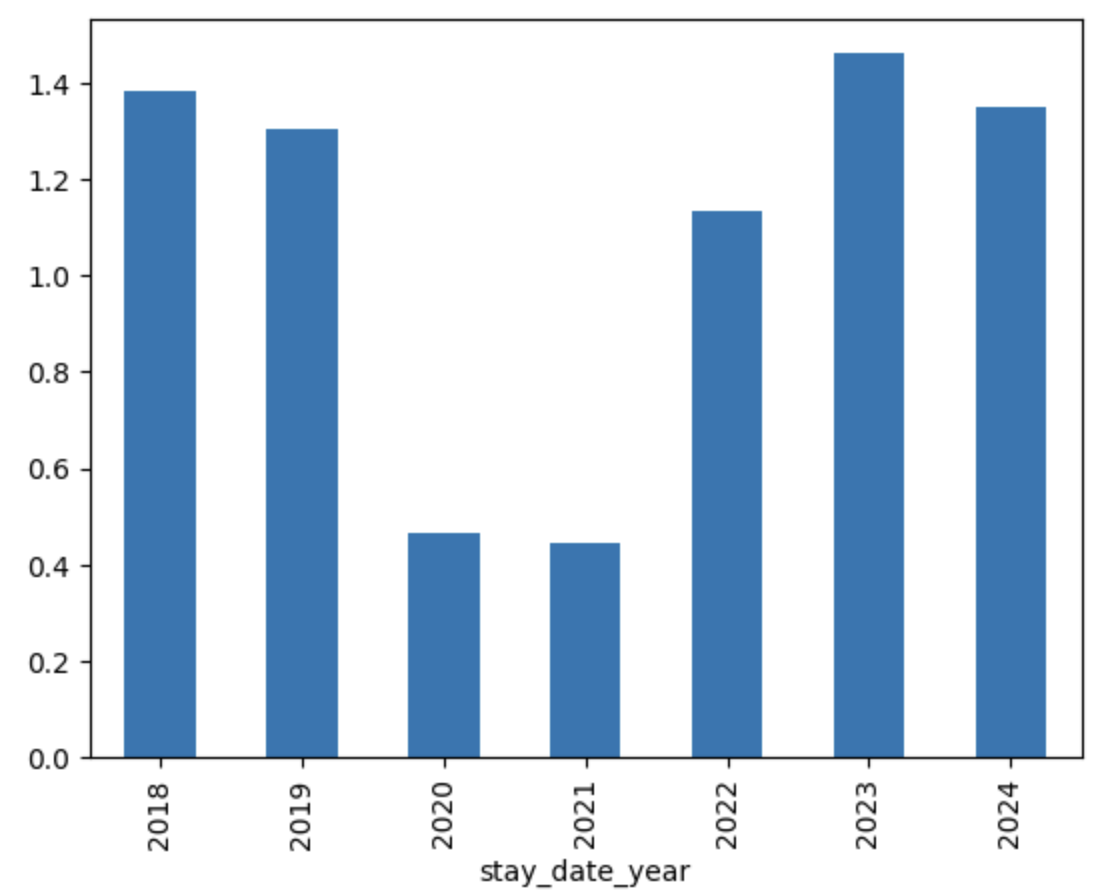
\includegraphics[width=1\textwidth, center]{revpar_target_year.png}
    \caption[Durchschnittlich normierte RevPAR-Werte pro Jahr]{Durchschnittlich normierte RevPAR-Werte pro Jahr}
    \label{img:revpar_target_year}
\end{figure}

Eine bedeutsame Erkenntnis aus Abbildung \ref{img:revpar_target_year} ist, dass nicht alle Jahre gleich sind. Insbesondere weisen die Jahre 2020 und 2021 einen deutlich niedrigeren durchschnittlichen RevPAR auf als die anderen Jahre. Diese Unterschiede können auf verschiedene Faktoren zurückzuführen sein, wobei die Zeit der Covid-19-Pandemie einen wesentlichen Beitrag zu dieser Abweichung geleistet haben dürfte, da viele Hotels zu dieser Zeit vorübergehend schließen mussten. Es wäre daher unangemessen, diese Informationen in das Modell einzubeziehen, da sie den Datensatz verfälschen würden. Da die Spalte 
\emph{stay\_date\_year}außer Ausreißern keine weiteren relevanten Informationen bietet, wird dieses Feature im weiteren Verlauf aus dem Datensatz entfernt.
\newline
\newline
Des Weiteren soll mit derselben Methodik überprüft werden, ob die Features
\newline 
\emph{stay\_date\_weekDayName}, \emph{stay\_date\_monthName} und \emph{holiday} einen signifikanten Einfluss auf den normierten RevPAR haben.

\newpage
\begin{figure}[h]
    \centering
    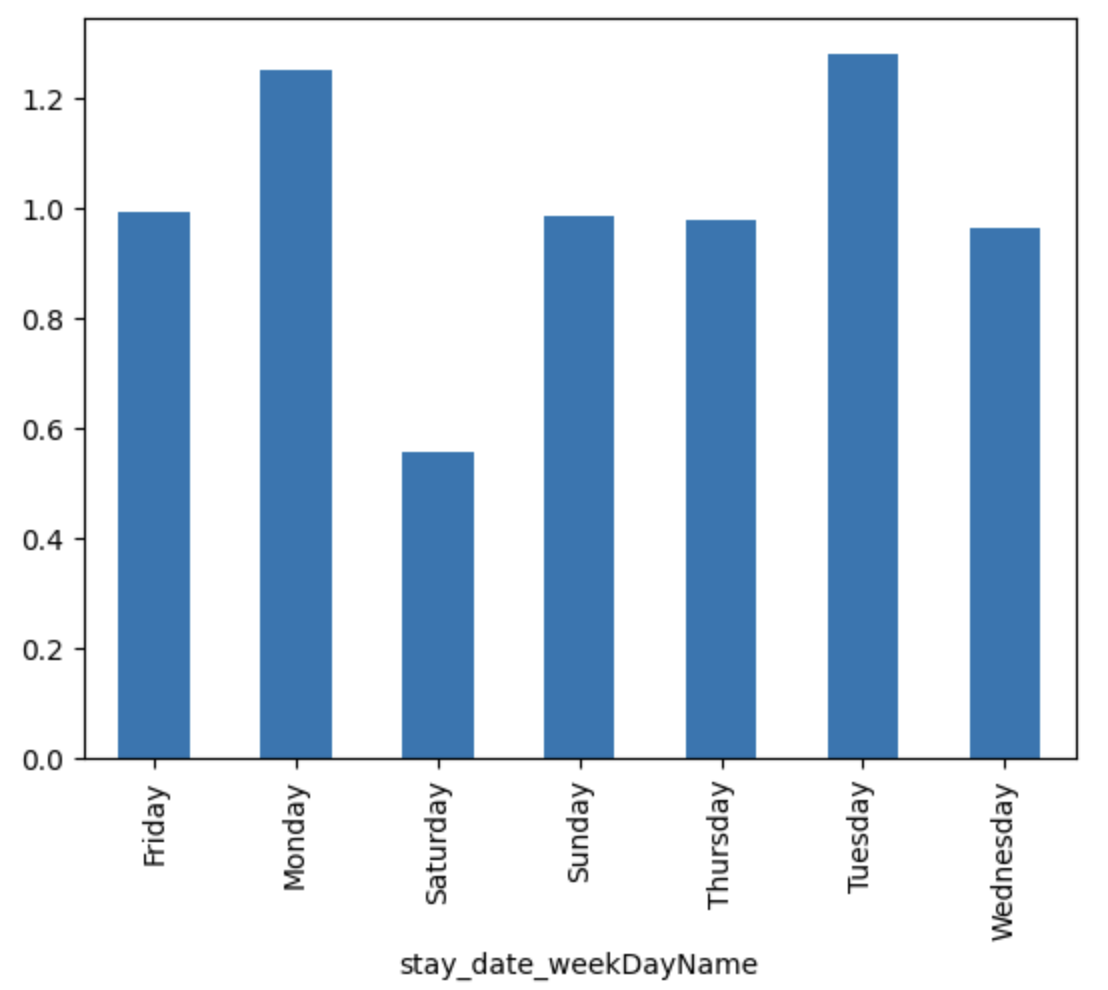
\includegraphics[width=0.6\textwidth, center]{revpar_target_week.png}
    \caption[Durchschnittlich normierte RevPAR-Werte pro Tag]{Durchschnittlich normierte RevPAR-Werte pro Tag}
    \label{img:revpar_target_week}
\end{figure}

\begin{figure}[h]
    \centering
    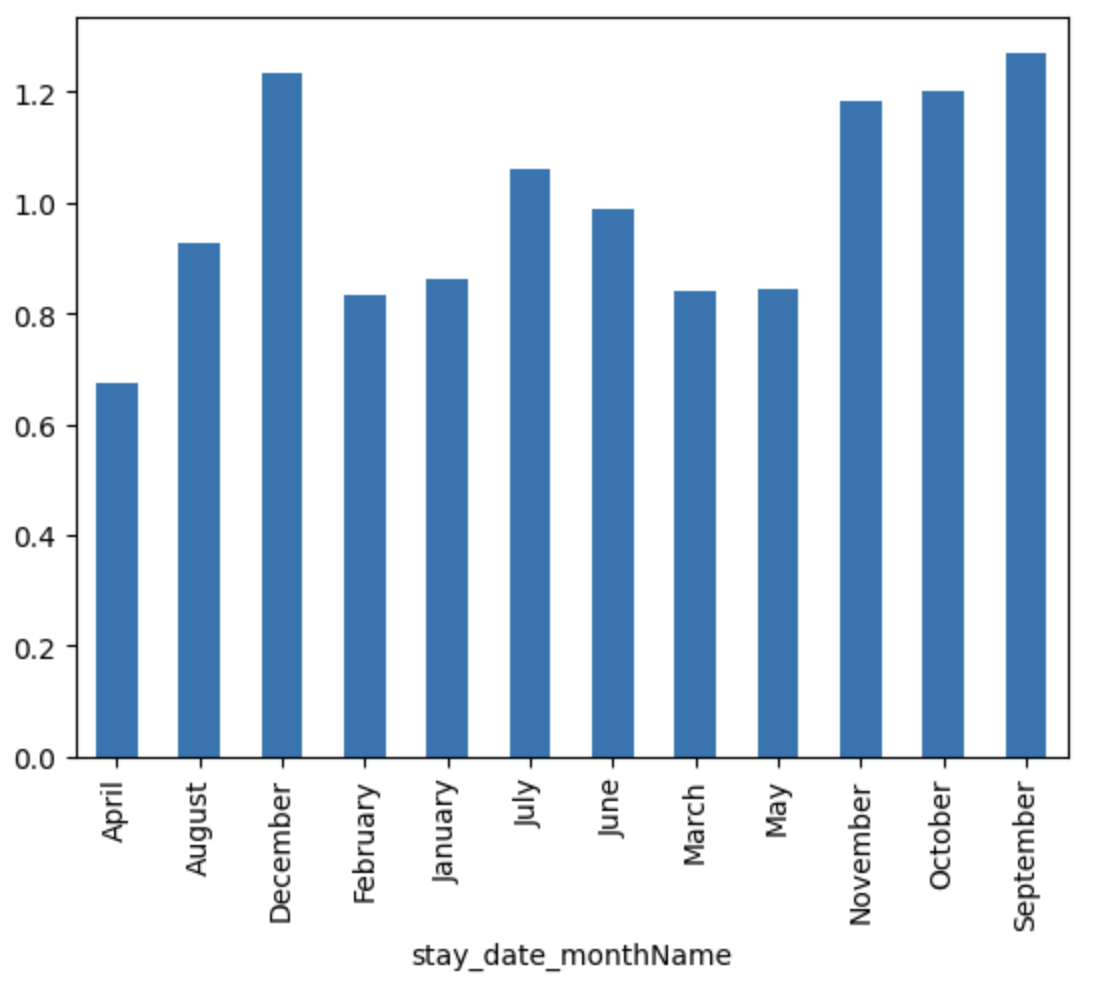
\includegraphics[width=0.6\textwidth, center]{revpar_target_month.png}
    \caption[Durchschnittlich normierte RevPAR-Werte pro Monat]{Durchschnittlich normierte RevPAR-Werte pro Monat}
    \label{img:revpar_target_month}
\end{figure}

\newpage

\begin{figure}[h]
    \centering
    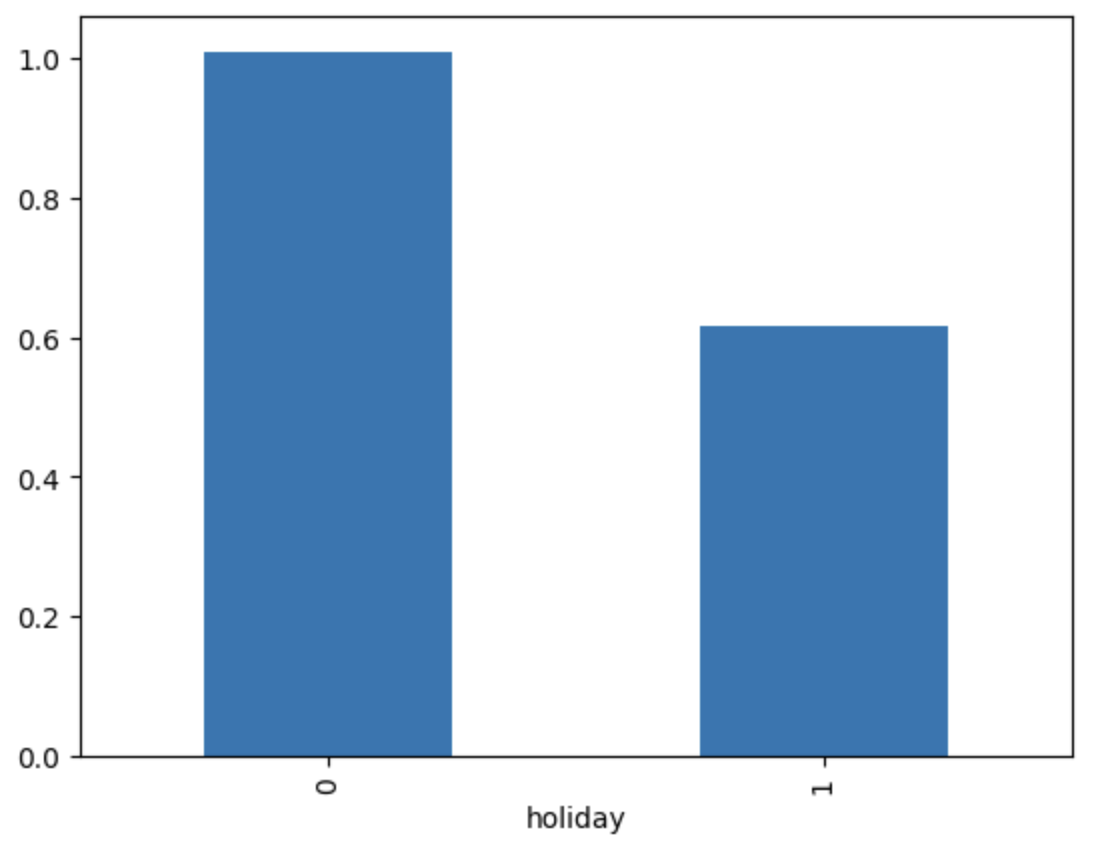
\includegraphics[width=0.6\textwidth, center]{revpar_target_holiday.png}
    \caption[Durchschnittlich normierte RevPAR-Werte Ferientage vs. nicht-Ferientage]{Durchschnittlich normierte RevPAR-Werte Ferientage vs. nicht-Ferientage}
    \label{img:revpar_target_holiday}
\end{figure}

Anhand der Abbildungen \ref{img:revpar_target_week}, \ref{img:revpar_target_month} und \ref{img:revpar_target_holiday} lässt sich erkennen, dass jedes dieser Features einen signifikanten Einfluss auf den normierten RevPAR hat und daher im Datensatz beibehalten werden sollte.
\newline 
\newline
Zum Abschluss sollen noch die Spalten \emph{scaled\_current\_adr}, \emph{scaled\_current\_revpar} und \emph{occupancy} auf ihren Einfluss überprüft werden. Hierzu wird im Folgenden eine Korrelationsmatrix erstellt, um die Korrelation dieser Spalten mit dem normierten RevPAR zu bestimmen.

\begin{figure}[h]
    \centering
    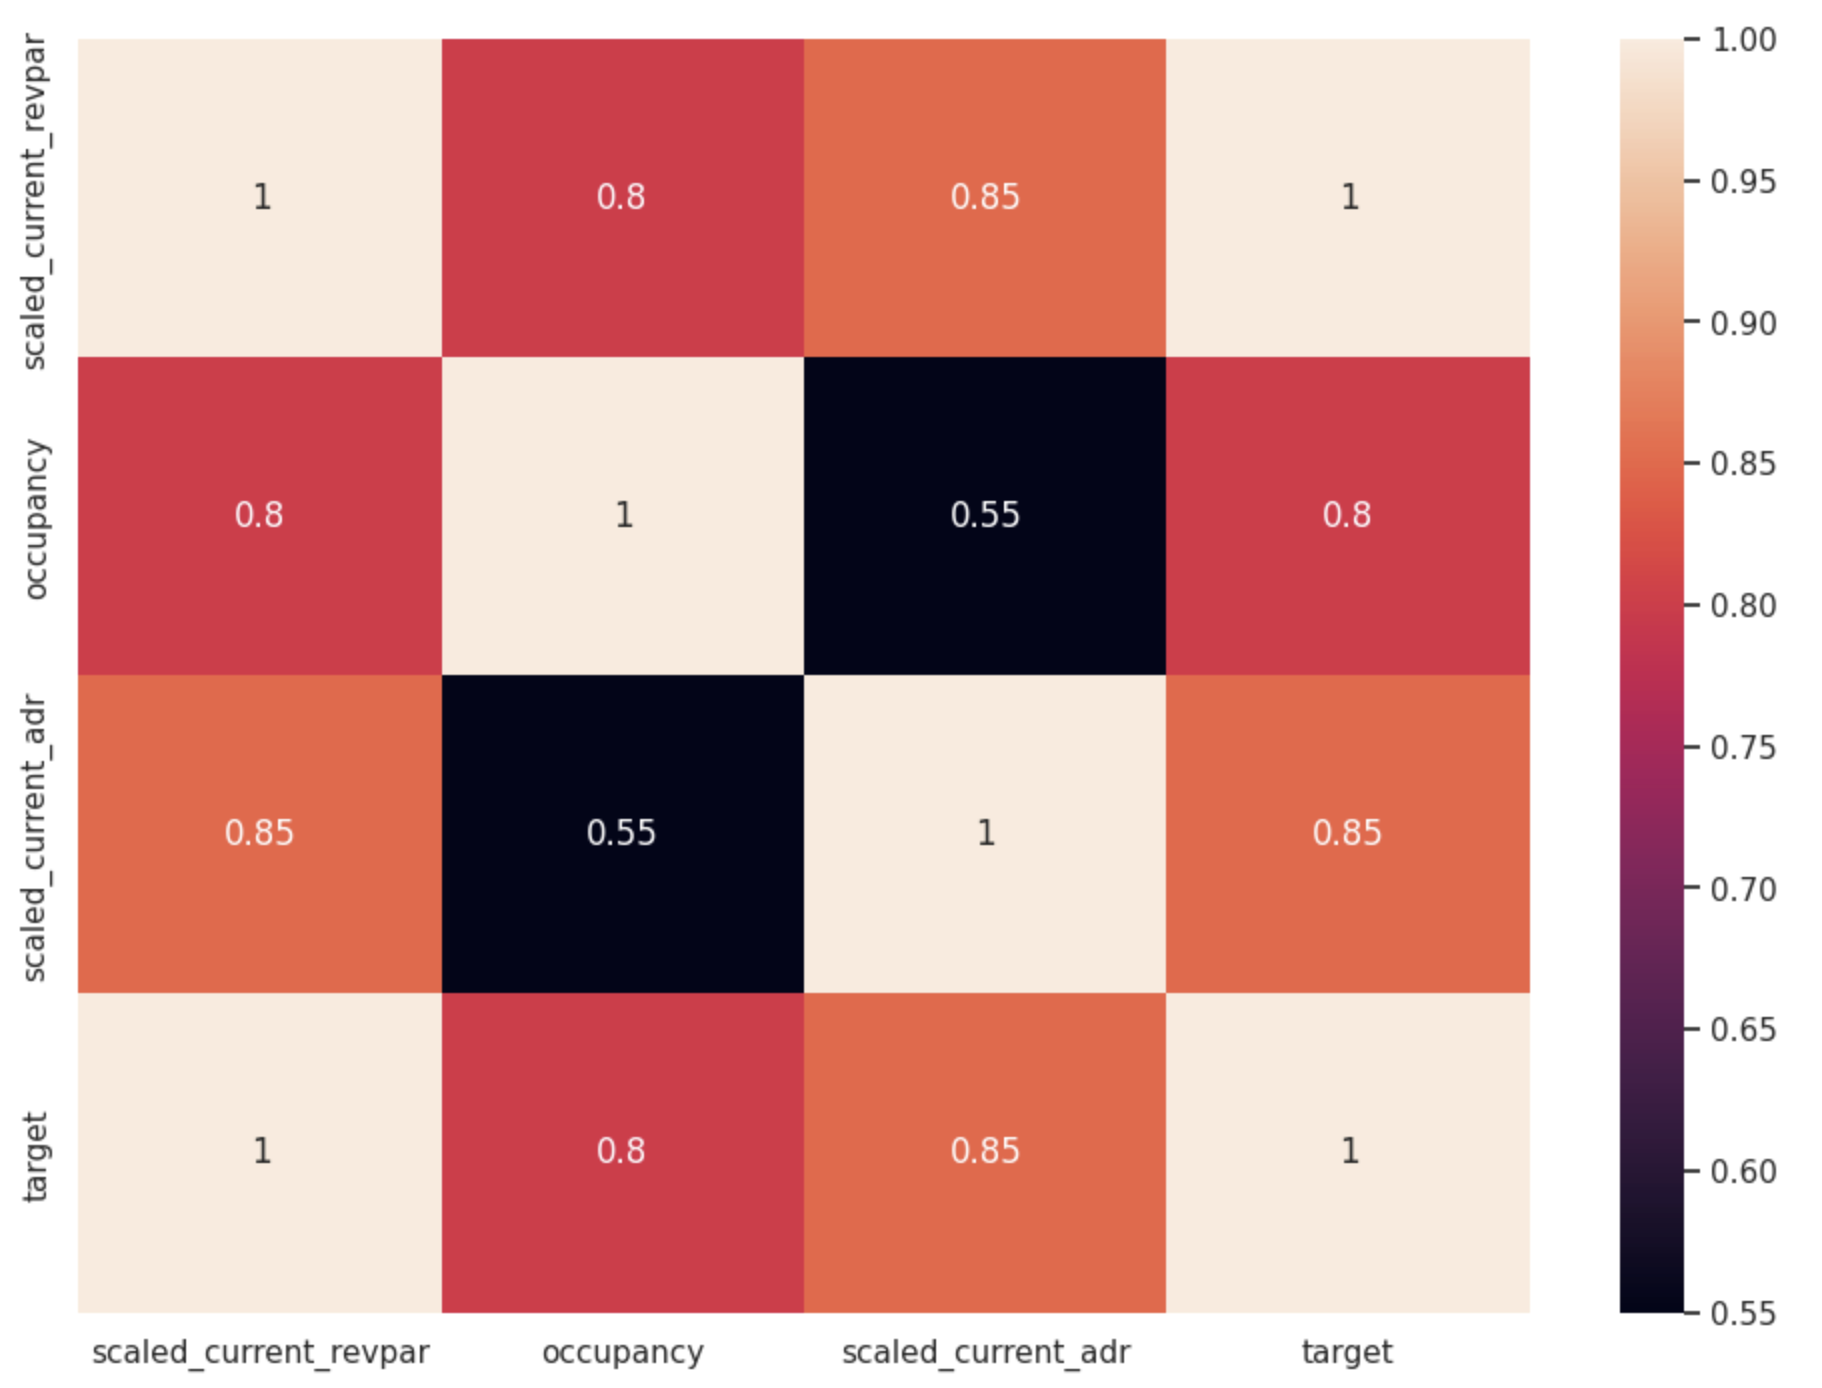
\includegraphics[width=0.6\textwidth, center]{revpar_corr.png}
    \caption[Korrelationsmatrix der verbleibenden Spalten]{Korrelationsmatrix der verbleibenden Spalten}
    \label{img:revpar_corr}
\end{figure}

Bei Betrachtung der unteren Zeile \emph{target} ist festzustellen, dass alle aufgelisteten Features eine signifikante Korrelation zur Zielvariable aufweisen. Daher sollten sie auch im Datensatz berücksichtigt werden.
\newline 
\newline 
Der resultierende Datensatz, welche nach der Entfernung der Ausreißer und unnötigen Feature entsteht sieht wie folgt aus:

\begin{figure}[h]
    \centering
    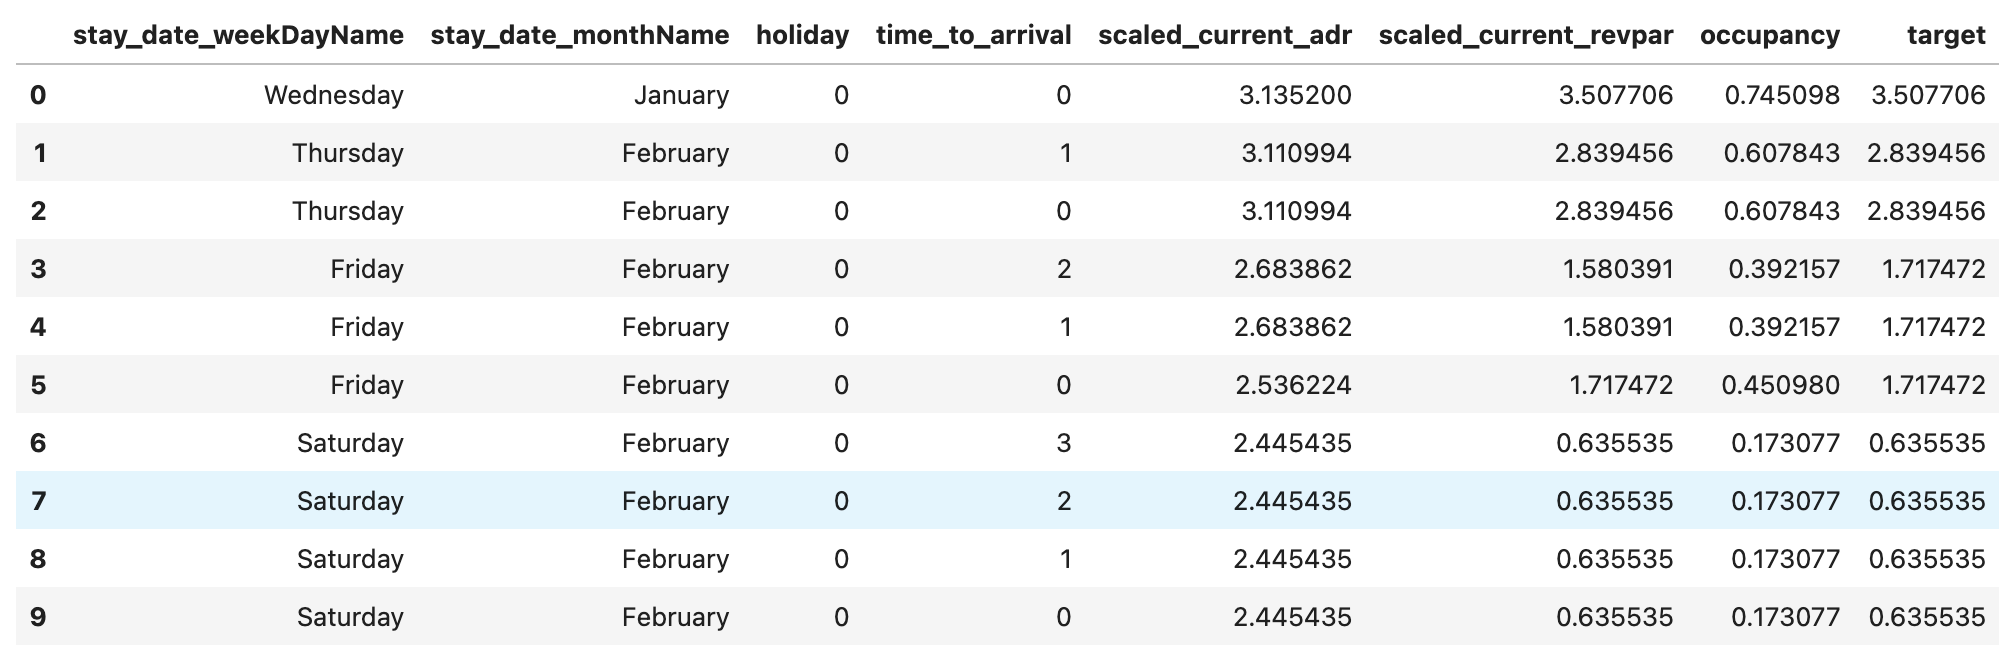
\includegraphics[width=1\textwidth, center]{revpar_df.png}
    \caption[Finaler Datensatz für das RevPAR-Modell]{Finaler Datensatz für das RevPAR-Modell}
    \label{img:revpar_df}
\end{figure}
